\newcommand{\caret}{{\large\textbf{\textasciicircum}}}

\section{Rudimant-Kompiler und Laufzeitsystem}

Der Rudimant-Kompiler übersetzt Regeldateien mit Extension \texttt{.rudi} in
Java-Dateien. Dazu braucht er eine Ontologie, in der die RDF Klassen und
Properties, die im \texttt{.rudi}-Code verwandt werden, spezifiziert sind.

Im Fall des POC liegen die Quelldateien in \texttt{src/main/rudi} und die
dazugehörende Ontologie in \texttt{src/main/resources/ontology}. Damit HFC
die Ontologie benutzen kann, muss sie im ntriples-Format vorliegen. Die
derzeitige Ontologie wird mit Protégé erstellt und aus dem OWL-XML Format
mit Hilfe des \texttt{rapper}-Tools in eine \texttt{.nt} ntriples Datei
übersetzt. \texttt{rapper} ist Teil des Ubuntu-Package \texttt{raptor2-utils},
das Script \texttt{ntcreate} im \texttt{poc} Verzeichnis updated alle nicht
aktuellen \texttt{.nt} Files aus den \texttt{.owl} Versionen.

Weitere settings, die für die Kompilation wichtig sind, finden sich in der
Datei \texttt{herbea.yml}, die von \texttt{compile} Skript benutzt wird. Auch
hier sind alle relativen Pfade relativ zum Verzeichnis, in dem die
\texttt{.yml} Datei liegt.

Für standalone Mockup-Tests kann der POC auch isoliert mit dem \texttt{run.sh}
script gestartet werden, die ``Sensordaten'' werden dann nach und nach in
der main-Methode eingespielt.

Der folgende Text ist leider unvollständig und muss noch ergänzt werden. Für
die meisten Konstrukte gibt es einige Beispiele in den \texttt{rudi}
Quelldateien.

\subsection{Rudimant Regeln}

%{\Huge TODO: testen, ob alle Beispiele so funktionieren, wie sie sollen !!!!!!}

\subsubsection{Externe Funktionen und Variablen}
\label{rudimant-global}

Für Funktionen, die nicht oder nur umständlich in rudi-Code implementiert
werden können, sollte der Nutzer eine Javaklasse \texttt{MyAgent} von der
abstrakten Klasse \texttt{Agent} ableiten. Diese Klasse wird als
\emph{Wrapper-Klasse} bezeichnet. Funktionen und Variablen, die in
dieser Klasse deklariert wurden und später im rudi-Code benutzt werden sollen,
müssen mit vollständiger Typangabe in einer Datei \texttt{MyAgent.rudi}
deklariert werden, sodass die Typinferenz von rudimant sie korrekt
berücksichtigen kann (zur Syntax siehe \ref{rudimant-Typinferenz}).

Die Klasse \texttt{MyAgent} inklusive Packagenamen muss in der config.yml Datei
eines Projektes unter dem Eintrag \texttt{wrapperClass} spezifiziert werden, um
im Compile-Schritt einen Effekt zu zeigen. Rudimant nutzt die Klasse
\texttt{MyAgent} dann als Superklasse der im Compile-Schritt angegebenen Datei
im rudi-Format und verlinkt Funktionsaufrufe und Variablennutzungen in allen
untergeordneten rudi-Dateien auf diese, sodass korrekte Aufrufe im
resultierenden Java-Code gewährleistet sind.

\subsubsection{RDF Zugriffe, funktionale vs. relationale Properties}

\begin{table}[htbp]
  \centering
\begin{small}
\begin{minipage}[t]{0.35\textwidth}
\begin{verbatim}
Child c;
String name = c.name;
c.name = "new name";
Set middle = c.middleNames;
c.middleNames += "John";
c.middleNames -= "James";
\end{verbatim}
\end{minipage}
\begin{minipage}[t]{0.6\textwidth}
\begin{verbatim}

String name = (String)c.getValue("<upper:name>");
c.setValue("<upper:name>", "new name");
Set middle = (Set<Object>)c.getValue("<upper:middleNames");
c.add("<upper:middleNames", "John");
c.remove("<upper:middleNames", "James");
\end{verbatim}
\end{minipage}
\end{small}
  \caption{Beispiele für RDF Property-Zugriff}
  \label{tab:property-access}
\end{table}


Durch die Verbindung zu \texttt{hfc} während des Compile-Vorganges hat rudimant
vollen Zugriff auf die Datenbank und kann nicht nur Rdf-Objekte anhand ihrer
Typen erkennen, sondern auch erkennen, wann ein Feldzugriff auf ein Rdf-Objekt
erfolgt und ihn in solchen Fällen in einen Zugriff auf die Datenbank
umwandeln. Dies ist sowohl für Zugriffe auf Properties als auch für Änderungen
ihres Inhalts möglich und lässt sich, sofern dies in der verwendeten Ontologie
korrekt möglich ist, beliebig oft hintereinander ausführen.

Sowohl die Verwendung von relationalen als auch die von funktionalen Prädikaten
ist erlaubt. Diese ändern die Aufrufe im rudi-Code jedoch grundsätzlich nicht,
da rudimant selbst inferiert, ob ein Zugriff auf die Datenbank ein einfaches
Objekt oder ein Set von Objekten zurückgibt. Lediglich die weitere Nutzung
dessen, was abgerufen wurde, muss sich (selbstverständlich) an die Art des
Ergebnisses des Rdf-Zugriffes anpassen. Versucht man allerdings, den Wert eines
relationalen

Die beiden Operatoren \texttt{+=} und \texttt{-=} sind in rudimant
überladen. Sie können sowohl wie in Java zum Rechnen mit Integer, float und
double verwendet werden, als auch im Zusammenspiel mit Sets und
Listen. \texttt{a += b} wird hierbei in \texttt{a.add(b)} umgewandelt,
\texttt{a -= b} resultiert in \texttt{a.remove(b)}.

\subsubsection{Regeln und Labels}

\begin{small}
\begin{verbatim}
introduction:
  if (introduction){
    if (user.unknown){
      ask_for_name:
        if (talkative) {
          askForName();
        }
    } else {
      greetUser();
    }
  }
\end{verbatim}
\end{small}

Das Kernstück von rudimant sind die Dialogregeln. Eine Regel beginnt mit ihrem
Namen, einem möglichst aussagekräftigen Label, gefolgt von einem
Doppelpunkt. Anschließend folgt ein if-statement. Die Clause des Statements
drückt die Bedingung aus, unter der die Regel ausgeführt werden soll, im Body
steht der auszuführende Code.

Auch eingeschachtelte \texttt{if}-Abfragen können mit Labels versehen werden.
Die Labels dienen einerseits zum debuggen des Codes, da im generierten Code
Funktionalität enthalten ist, um den Agenten zur Laufzeit zu debuggen. Dazu
kann man zur Zeit zwei API-Funktionen von \texttt{Agent} benutzen, nämlich
\texttt{logRule(String rulename)} und \texttt{logAllRules()}

Der Output des Loggers wird dann das Label jeder Regel, die evaluiert wird,
zusammen mit der Auswertung der Bedingung und den Werten aller booleschen
Basisterme, die in der Bedingung vorhanden sind, angeben.

\todo[inline]{Bsp debugging-output}

\subsubsection{Ausstieg aus Regeln}

Es gibt mehrere Möglichkeiten, die Regelverarbeitung lokal oder ganz
abzubrechen. Aus einer gelabelten Regel kann man z.B. mit
\verb|break label_name;| aussteigen. Alle danach folgenden Regeln werden dann
weiter verarbeitet.

Bricht man die Verarbeitung mit \texttt{cancel} ab, wird keine der in
der Datei folgenden Regeln mehr angewandt, bei \texttt{cancel\_all} wird
keine nachfolgende Regel, weder lokal, noch auf höheren Ebenen, angewandt.

Um \texttt{propose} oder \texttt{timeout} Blöcke zu verlassen, muss
\texttt{return} benutzt werden, da dies normale Funktionsblöcke sind.

\subsubsection{Propose}

\subsubsection{Struktur einer Datei im rudi-Format}

Anders als Java stellt rudimant nicht den Anspruch, dass die Einträge in einer
Datei in irgendeine Form von übergeordneter Struktur gefasst werden. Die Regeln
können ebenso wie Funktionsdeklarationen direkt in die Datei geschrieben
werden. Dasselbe gilt für jede Art valider (Java-) Statements, wie etwa
Zuweisungen, for-Schleifen usw.. Rudimant wird bei der Kompilation eine
Java-Klasse erstellen, in die es die Funktionen sowie die Regeln, zu Funktionen
transformiert, einträgt. Alle weiteren Statements werden in der korrekten
Reihenfolge in die erzeugte Methode process() verschoben, wobei generierte
Aufrufe an die Regelfunktionen zwischen ihnen gewährleisten, dass die Regeln
und Statements in der Reihenfolge ausgeführt werden, die im rudi-Code
spezifiziert war. Dies ermöglicht also, nicht in Regeln gefasste
Abbruchbedingungen einzubauen, unter denen die Ausführung der ganzen Datei -
und möglicher importierter Dateien - sofort beendet werden soll.

Datei-global deklarierte Variablen werden als Klassenvariablen angelegt.

\subsubsection{Dialogakte und Evaluation mittels \caret}
\label{sub:caret}

\begin{small}
\begin{verbatim}
emitDA(#Inform(Answer, what=^solution));
\end{verbatim}
\end{small}
Eine wichtige Aufgabe eines Dialogsystems ist zweifellos die Ausgabe von
Dialogakten, die von der Generierungskomponente zu Kommunikation mit dem Nutzer
verarbeitet werden können. In rudimant ist die Funktion \texttt{emitDA} hierfür
zuständig.

Argument von \texttt{emitDA} ist ein Dialogakt in der oben gezeigten Form. Dass
es sich bei \texttt{Inform}\verb|(...)| nicht um einen Funktionsaufruf, sondern
um einen Dialogakt handelt, wird hier und an allen anderen Stellen, an denen
man einen Dialogakt benutzen möchte, durch das \verb|#|
gekennzeichnet. Rudimant wird so erkennen, dass im Java-Code eine neue Instanz
der Klasse DialogueAct mit den entsprechenden Modifikationen erstellt werden
muss. Hierbei kommt dem Marker \caret{} eine besondere Bedeutung zu: Per
default werden alle in den Klammern angegebenen Argumente, egal, ob sie rechts
oder links eines $=$ stehen, als Strings an den neuen DialogueAct
übergeben. Möchte man explizit den Inhalt einer Variablen oder eines Ausdrucks
übergeben, so ist die Benutzung von \caret{} vor der entsprechenden rechten
Seite einer Zuweisung notwendig, die dafür sorgt, dass der Ausdruck evaluiert
wird, und nicht als atomares Symbol interpretiert.

\subsubsection{Typinferenz und überladene Vergleichsoperatoren}
\label{rudimant-Typinferenz}

Rudimant erlaubt statische Typzuweisungen sowie Casting, beides ist jedoch
nicht zwingend notwendig.

Ist beispielsweise der Typ der rechten Seite einer Variablendeklaration mit
Zuweisung bekannt oder inferierbar, so ist es nicht notwendig, den Typ der
Variablen explizit anzugeben.

\begin{table}[htbp]
  \centering
  \begin{small}
    \begin{BVerbatim}
      if (! c.user.personality.nonchalance){ ... }
    \end{BVerbatim}

    {\Large$\Downarrow$}\\

    \begin{BVerbatim}
      if (!((((c != null) && (c.user != null))
             && (c.user.personality != null))
            && (c.user.personality.nonchalance != null))) {
         ...
      }
\end{BVerbatim}
\end{small}

\caption{Übersetzung komplexer Zugriffe}
\label{tab:multi-predaccess}
\end{table}
\vspace*{10pt}

Als zeitsparendes Feature bietet rudimant insbesondere das automatische
Vervollständingen von bool'schen Ausdrücken in den Clauses von if, while und
for an. Da in diesem Fall bekannt ist, dass das Ergebnis boolean sein muss,
ergänzt rudimant automatisch den Test auf die Existenz eines Objektes in der
Clause, sollte dieses nicht Typ boolean sein. Bei Feldzugriffen testet es für
jeden Teilzugriff, dass das erhaltene Objekt nicht null ist, um einer
NullPointerException zur Laufzeit des generierten Codes vorzubeugen.

Die Vergleichsoperatoren in rudimant sind überladen. Neben den aus Java bekannten Anwendungen als Vergleichsoperatoren können sie auch auf Dialogakte angewendet werden. In diesen Fällen werden sie zu Subsumptionsoperatoren.

\begin{table}[htbp]
  \centering
  \begin{footnotesize}
    \begin{minipage}{0.3\textwidth}
\begin{verbatim}
if (sa <= #Question){
  ...
}
\end{verbatim}
    \end{minipage}
    \begin{minipage}{0.5\textwidth}
\begin{verbatim}
if (sa.isSubsumedBy(new DialogueAct("Question")) {
  ...
}
\end{verbatim}
    \end{minipage}
  \end{footnotesize}

  \caption{Überladene Vergleichsoperatoren}
  \label{tab:overloaded-comparison}
\end{table}

\paragraph{Rudimant Typinformationen zur Verfügung stellen}

In manchen Fällen, wie etwa der Benutzung von außerhalb der rudi-Dateien
deklarierten Funktionen und Variablen, ist es notwendig, rudimant Informationen
über Typen zu geben. Dabei gilt folgendes Schema, nach dem Typen an beliebiger
Stelle, für gewöhnlich jedoch in der Datei MyAgent.rudi (siehe
\ref{rudimant-global}) deklariert werden können:


\begin{table}[htbp]
  \centering
  \small
  \begin{tabular}{lp{.45\textwidth}}
    \texttt{myType someVariable;}
    &  es gibt die Variable myVariable vom Typ \texttt{myType} \\

    \texttt{myType someFunction(typeA a, typeB b);}
    &  Funktion someFunction nimmt Argumente vom Typ \texttt{typeA} und
      \texttt{typeB} und gibt ein Objekt vom Typ \texttt{myType} zurück (void =
      void) \\

    \texttt{[type]. myType Function(typeA a);}
    & Funktionsdeklaration wie oben; die Funktion muss auf einem Objekt der
      Klasse \texttt{type} aufgerufen werden. Generics sind eingeschränkt
      erlaubt, mit T als festgelegtem Namen der Parameter-Klasse,
      Beispiel:\newline\texttt{[List<T>]. T get(int i);}
  \end{tabular}

  \caption{Typinferenz}
  \label{tab:typeinference}
\end{table}

Wichtig ist: Diese Deklarationen werden nur für die Berechnung der Typen durch
rudimant angegeben und werden nicht in den kompilierten Code
übernommen. Insbesondere Zeilen wie \texttt{int i;} oder \texttt{void
  someFunction();} entsprechen damit nicht einer gleich aussehenden Deklaration
im Java-Code. Falls es einen Grund geben sollte, dass die Zeilen als im
Compile-Ergebnis als dringend erforderlich betrachtet werden, hilft die in
Kapitel \ref{rudi-verbatim} beschriebene Methode.

%\subsubsection{Überladene Vergleichsoperatoren und Tests}
%Dies überschneidet sich in großen Teilen mit dem Doku-Teil zur Typinferenz; wurde dort untergebracht

\subsubsection{Funktionale Konstrukte (lambda)}

Rudimant erlaubt die Verwendung von lambda-Konstrukten. Im moment können sie
aber nur für die Implementierung von \texttt{Predicate}
resp. \texttt{Comparator} in den im folgenden angegebenen vier
Funktionen. Diese Funktionen sind in \texttt{Agent} vordefiniert. Ein
einfaches Beispiel zum Filtern von Objekten mit einer Subtyprelation wäre:

\begin{verbatim}
des = filter(agent.desires, (d) -> ((Desire)d) <= UrgentDesire);
\end{verbatim}


\begin{table}[htbp]
  \centering
  \begin{small}
\begin{verbatim}
boolean contains(Collection coll, Predicate pred);
boolean all(Collection coll, Predicate pred);
List<Object> filter(Collection coll, Predicate pred);
List<Object> sort(Collection coll, Comparator c);
\end{verbatim}
  \end{small}

  \caption{Funktionen, die mit Lambda-Ausdrücken benutzt werden können.}
  \label{tab:lambda-functions}
\end{table}

\subsubsection{\texttt{import}}

\texttt{import} ist ein Schlüsselwort in rudimant. Eine Zeile ''\texttt{import
  File;}'' auf globaler Ebene, an einer beliebigen Stelle zwischenn den Regeln,
bedeutet die Inklusion der Datei File.rudi an exakt dieser Stelle. Hiermit wird
zum einen erreicht, dass rudimant auch diese Datei zu ausführbarem Java-Code
kompiliert, sodass nicht alle Dateien eines Projektes separat kompiliert werden
müssen. Zum anderen wird das vollständige Regelinventar der Datei an der
entsprechenden Stelle im Java-Code mithilfe ihrer process-Methode aufgerufen
und durchgearbeitet.

\texttt{import} ermöglicht es also, das Regelinventar für ein Projekt auf
mehrere Dateien bzw. mehrere Module aufzuteilen und diese zusammenzustecken,
sodass ein einziger Aufruf ausreicht, um sie zu kompilieren und später auch, um
die Auswertung der Regeln anzustoßen. Dies ist nicht nur nützlich zur
Übersichtlichkeit und Strukturierung des Projektes, sondern fördert auch die
Modularität, da verschiedene 'Unterbäume' der \texttt{import}-Hierarchie leicht
ausgeklinkt oder aus anderen Projekten wiederverwendet werden können.

\subsubsection{Java-Code verbatim im Regelfile} \label{rudi-verbatim}

Rudimant verarbeitet eine Regelsprache, die mit voller Absicht nur
eingeschränkte Java-Funktionalitäten zur Verfügung stellt. Was in rudi-Code
nicht umzusetzen ist, sollte in Funktionen in die übergeordnete Java-Klasse
wandern (vgl. \ref{rudimant-global}).

Für Fälle, in denen dies nicht genügt und vor Ort eine Funktionalität benötigt
wird, die rudimant nicht parsen oder nicht richtig darstelllen kann, ist eine
verbatim-Umgebung vorgesehen. Alles, was innerhalb der Zeichenfolgen \verb|/*@|
und \verb|@*/| steht, wird behandelt wie ein mehrzeiliges Java-Kommentar, wird
also in genau diesem Aussehen in den resultierenden Code übertragen. Dabei
werden die klammernden Zeichenfolgen ausgelassen.

Diese Funktionalität kann insbesondere dazu benutzt werden, am Anfang einer
\texttt{rudi} Datei Java-Klassen zu importieren, die im kompilierten Code
gebraucht werden.

\subsection{Architektur von Rudimant}

In der Abbildung~\ref{fig:architecture} ist die Gesamtarchitektur skizziert.

\begin{figure}[htbp]
  \centering
  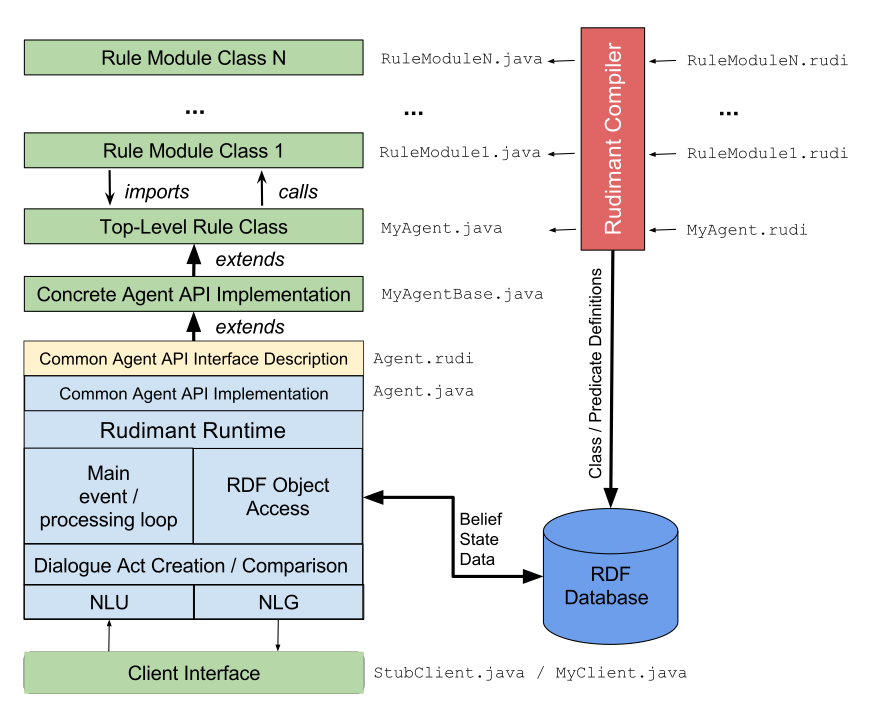
\includegraphics[width=.8\textwidth]{RudimantStructure.png}
  \caption{Gesamtarchitektur von Rudimant}
  \label{fig:architecture}
\end{figure}

Rudimant besteht aus einem Compiler und einem Laufzeitsystem. Daraus wird eine
konkrete Applikation, indem zunächst eine spezielle Java-Klasse, die sogenannte
\emph{Wrapper-Klasse}, von der Klasse \texttt{Agent} abgeleitet wird. Diese
kann Implementierungen von \texttt{Agent} erweitern oder
überschreiben. Außerdem können eigene Java-Methoden für die Benutzung in den
Regelfiles zur Verfügung stellen, die sich nicht ohne weiteres in \texttt{rudi}
Dateien implementieren lassen (komplexe Queries an die Datenbank, etc.). Im
Bild ist dies \texttt{MyAgent.java}.

Damit der Compiler diese Funktionen kennt, müssen sie in der Datei
\texttt{MyAgent.rudi} deklariert werden. Sie beschreibt sozusagen das
Interface, auf das der \texttt{rudi} Quellcode zugreifen kann.

\todo{Das kann man doch in allen .rudi files}
Hier können auch statt der generischen Klasse \texttt{Rdf} die Klassen aus der
Ontologie spezifiziert werden, wenn diese genauer angegeben werden können. Das
hilft dem Kompiler bei der Typinferenz und dem richtigen Zugriff mit
RDF-Prädikaten.

Eine weitere wichtige Klasse ist \texttt{MyClient.java}, der die Kommunikation
mit der Außenwelt herstellt und das Laufzeitsystem von konkreten
Kommunikationsinterfaces abschirmt.

\subsection{Default-Funktionalität im Laufzeitsystem}
Alles was in \texttt{Agent} bereitgestellt wird. Die aktuelle Liste der
bereitgestellten Funktionen finden sich in \texttt{rudimant} unter
\texttt{src/main/resources/Agent.rudi}.

\begin{itemize}
\item timeouts
\begin{verbatim}
void newTimeout(String name, int millis);
boolean isTimedOut(String name);
void removeTimeout(String name);
boolean hasActiveTimeout(String name);
\end{verbatim}
\item Senden von Dialogakten an die Generierung
\begin{verbatim}
DialogueAct emitDA(int delay, DialogueAct da);
DialogueAct emitDA(DialogueAct da);
\end{verbatim}
\item Zugriff auf DialogAkte aus der Session
\begin{verbatim}
// my last outgoing resp. the last incoming dialogue act
DialogueAct myLastDA();
DialogueAct lastDA();

// did i say something like ta in this session (subsumption)? If so, how many
// utterances back was it? (otherwise, -1 is returned)
int saidInSession(DialogueAct da);
// like saidInSession, only for incoming dialogue acts
int receivedInSession(DialogueAct da);

boolean waitingForResponse();
void lastDAprocessed();
\end{verbatim}
\end{itemize}

%%% Local Variables:
%%% mode: latex
%%% TeX-master: "master"
%%% End:
